\chapter{これはchapter}
\section{これはsection}
我輩は猫である\footnote{こんな感じで脚注を書く}。

どこで生れたかとんと見当がつかぬ。何でも薄暗いじめじめした所でニャーニャー泣いていた事だけは記憶している。吾輩はここで始めて人間というものを見た。しかもあとで聞くとそれは書生という人間中で一番獰悪な種族であったそうだ。この書生というのは時々我々を捕えて煮て食うという話である。

\begin{tcolorbox}[breakable]
\begin{verbatim}
1  /* ここにはソースコードを書く */
2  #include<stdio.h>
3
4  int main(void)
5  {
6    printf("Hello, World!\n");
7    return 0;
8  }
9  /* breakableを付けるとこんな感じで改行にも対応できる */
\end{verbatim}
\end{tcolorbox}

\begin{shaded}
\begin{verbatim}
## ここにはコマンドを書く
$ echo "Hello, World!"
\end{verbatim}
\end{shaded}

図表はキャプションを付けたときに、先頭に「▲」や「▼」を付けるようにした。

\begin{table}[H]
  \centering
  \caption{表のサンプル}
  \begin{tabular}{|c|l|l|l|} \hline
    日本 & hoge & fuga & piyo \\ \hline
    アメリカ & foo & bar & baz \\ \hline
  \end{tabular}
  \label{table-sample}
\end{table}

\begin{figure}[H]
  \centering
  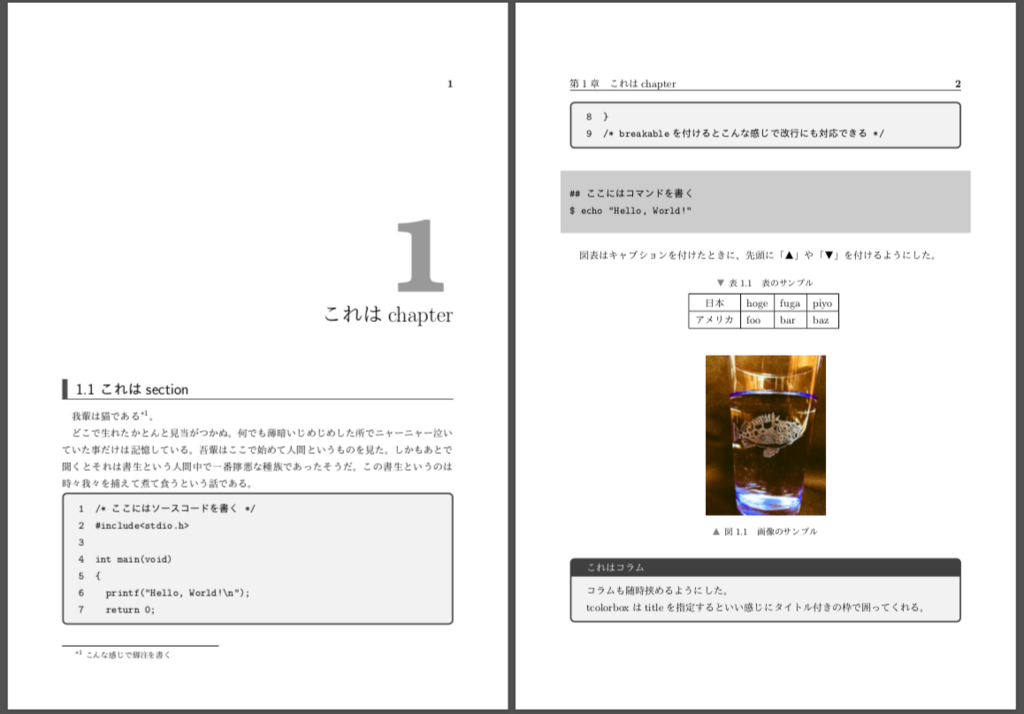
\includegraphics[width=4cm]{image/sample.png}
  \caption{画像のサンプル}
  \label{figure-sample}
\end{figure}

\begin{tcolorbox}[title=これはコラム]
  コラムも随時挟めるようにした。

  tcolorboxはtitleを指定するといい感じにタイトル付きの枠で囲ってくれる。
\end{tcolorbox}